\documentclass[aspectratio=169]{beamer}


\usepackage[utf8]{inputenc}
\usepackage{amsmath}
\usepackage{amsfonts}
\usepackage{amssymb}
\usepackage{graphicx}
\usepackage{ragged2e}  % `\justifying` text
\usepackage{booktabs}  % Tables
\usepackage{tabularx}
\usepackage{tikz}      % Diagrams
\usetikzlibrary{calc, shapes, backgrounds}
\usepackage{amsmath}
\usepackage{amssymb}
\usepackage{dsfont}
%%\usepackage{url}       % `\url
\usepackage{listings}  % Code listings
\usepackage[T1]{fontenc}
\font\myfont=cmr12 at 10pt


\usepackage{theme/beamerthemehbrs}

\author[Name]{Elanton Fernandes}
\subtitle{Active Learning Loop}
\title{Analysis of Active Learning Mechanism Applied to Language Models for Computer Assisted Short Answer Grading}
\institute[HBRS]{Hochschule Bonn-Rhein-Sieg}
\date{\today}
\subject{Test beamer}

% leave the value of this argument empty if the advisors
% should not be included on the title slide
\def\advisors{Prof. Dr. Paul G. Pl{\"o}ger, M.Sc Tim Metzler}

% \thirdpartylogo{path/to/your/image}


\begin{document}
{
\begin{frame}
\titlepage
\end{frame}
}


\section{Motivation}
\begin{frame}{Motivation}
	In universities with an increase in number of student every semester, the number of tests conducted also increases. This means that:
	\begin{itemize}
		\item The professor spends more time in correcting student exams than preparing for lectures.
		\item If students are not assigned full scores for on a test, they expect a meaningful feedback from the professor.
	\end{itemize}
\end{frame}
\begin{frame}{Motivation}
	Consider the following dummy scenario:
	\begin{itemize}
		\item 80 students enrolled in a class.
		\item Tests are conducted bi-weekly.
		\item Professor requires 15 minutes to evaluate one student test.
		\item Total time spent by the professor to evaluate all tests per week is 10 hours. 
	\end{itemize}
\end{frame}
\section{Problem Statement}
\begin{frame}{Problem Statement}
	%\framesubtitle{Problem Statement}
	\begin{itemize}
		\item To automate the evaluation of student tests while still keeping the oracle/professor in the loop.
		\item Allow the assignment of meaningful feedback to student answers indicating their mistakes.
	\end{itemize}
	
\end{frame}

\section{State of the Art}
\section{Approach}
\begin{frame}{Approach}
	\framesubtitle{Training cycle}
	\begin{figure}
		\centering
		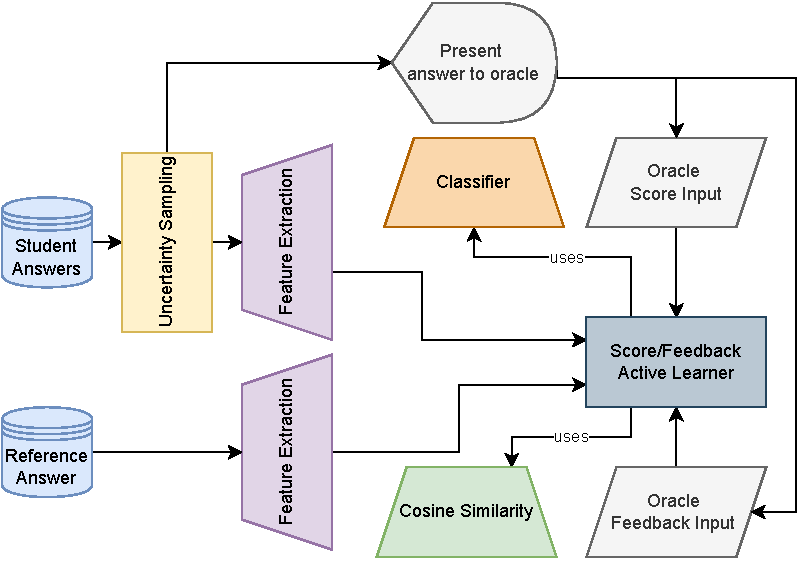
\includegraphics[scale = 0.65]{images/architecture_training.pdf}
		\label{fig:architecture train}
	\end{figure}
\end{frame}
\begin{frame}{Approach}
\framesubtitle{Prediction cycle}
\begin{figure}
	\centering
	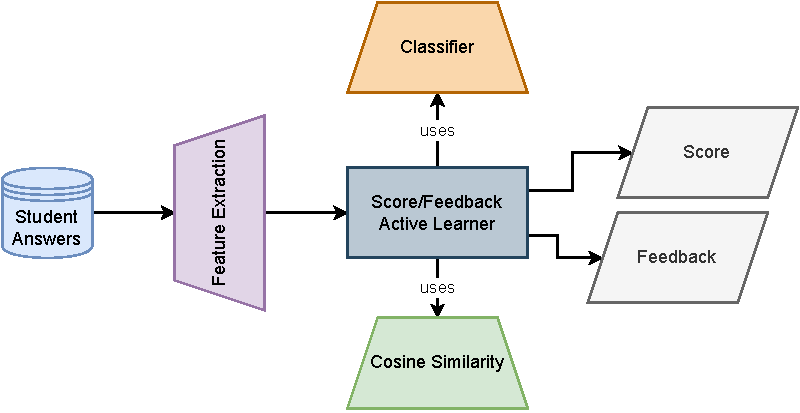
\includegraphics[scale = 0.65]{images/architecture_prediction.pdf}
	\label{fig:architecture predict}
\end{figure}
\end{frame}
\begin{frame}{Approach}
	\framesubtitle{Uncertainty Sampling}
	Uncertainty sampling is a query strategy that queries the instances about which it is least certain how to label. We use uncertainty sampling variant might query the instance whose prediction is the least confident:
	\begin{equation}
	\label{equation:uncertainty sampling}
	\scalebox{1.2}{$x_{LC} = argmin_{x} P({\hat{y}|x;\theta})$}
	\end{equation}
	Where $x$ is the feature, $y$ is the class label prediction, and $\hat{y} = argmax_y P({y|x;\theta})$ is the class label that has the largest posterior probability using model $\theta$.
\end{frame}
\begin{frame}{Approach}
\framesubtitle{Feature Extraction: Overview}
\begin{figure}
	\centering
	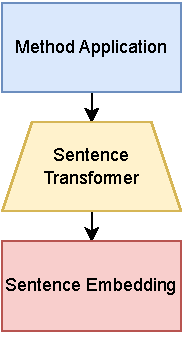
\includegraphics[scale = 0.65]{images/feature_extraction.pdf}
	\label{fig:feature extraction}
\end{figure}
\end{frame}
\begin{frame}{Approach}
\framesubtitle{Feature Extraction: Passage-based method}
\begin{figure}
	\centering
	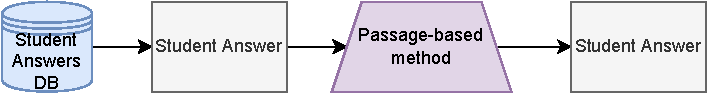
\includegraphics[scale = 0.65]{images/passage_FE_slides.pdf}
	\label{fig:passage fe slides}
\end{figure}
\end{frame}
\begin{frame}{Approach}
\framesubtitle{Feature Extraction: Sentence-based method}
\begin{figure}
	\centering
	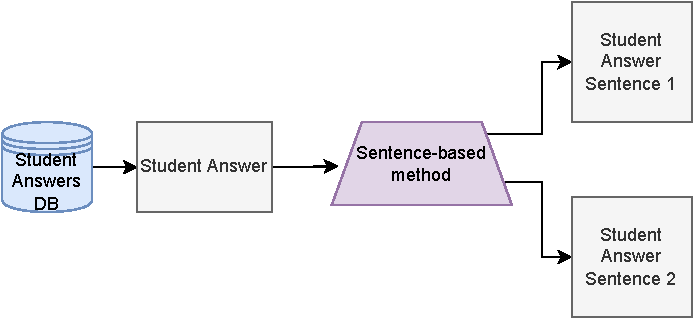
\includegraphics[scale = 0.65]{images/sentence_FE_slides.pdf}
	\label{fig:sentence fe slides}
\end{figure}
\end{frame}
\begin{frame}{Approach}
\framesubtitle{Feature Extraction: Chunk-based method}
\begin{figure}
	\centering
	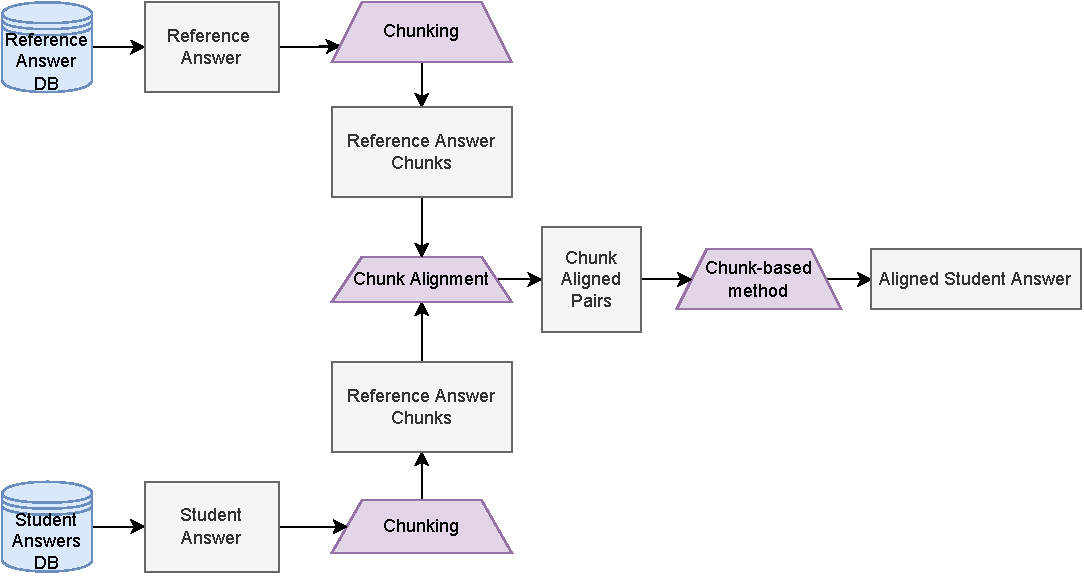
\includegraphics[scale = 0.5]{images/chunk_FE_slides.pdf}
	\label{fig:chunk fe}
\end{figure}
\end{frame}
\begin{frame}{Approach}
\framesubtitle{Feature Extraction: RDF-based method}
\begin{figure}
	\centering
	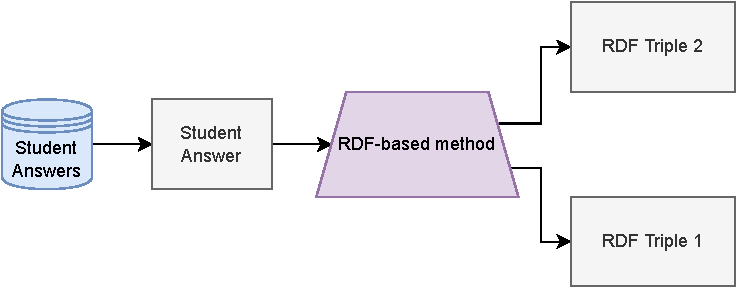
\includegraphics[scale = 0.65]{images/RDF_FE_slides.pdf}
	\label{fig:rdf fe}
\end{figure}
\end{frame}
\begin{frame}{Approach}
\framesubtitle{Language Models}
\begin{table}
	\begin{center}
		\begin{tabular}{ |c|c|c| }
			\hline
			Model: & Base model & Number \\&&Training tuples  
			\\ \hline 
			all-mpnet-base-v2\cite{SBERT} & 	microsoft/mpnet-base. &1.17B
			
			\\ \hline
			all-distilroberta-v1\cite{SBERT} & 	distilroberta-base &1.12B
			\\ \hline
			all-MiniLM-L12-v2\cite{SBERT} & 		microsoft/MiniLM-L12-H384-uncased &1.17B
			\\ \hline
			multi-qa-distilbert-cos-v1\cite{SBERT} & 	distilbert-base &214M
			\\ \hline
			all-MiniLM-L6-v2\cite{SBERT} & 		nreimers/MiniLM-L6-H384-uncased &1.17B
			\\ \hline
		\end{tabular}
		\caption{Displays pre-trained language models with their base model used in training and number of training tuples used\cite{SBERT}.}
		\label{table:language models}
	\end{center}
\end{table}
\end{frame}
\section{Results}
\begin{frame}{Results}
	\framesubtitle{Scores}
	\begin{table}
		\centering
		\resizebox{0.4\textwidth}{!}{% %
		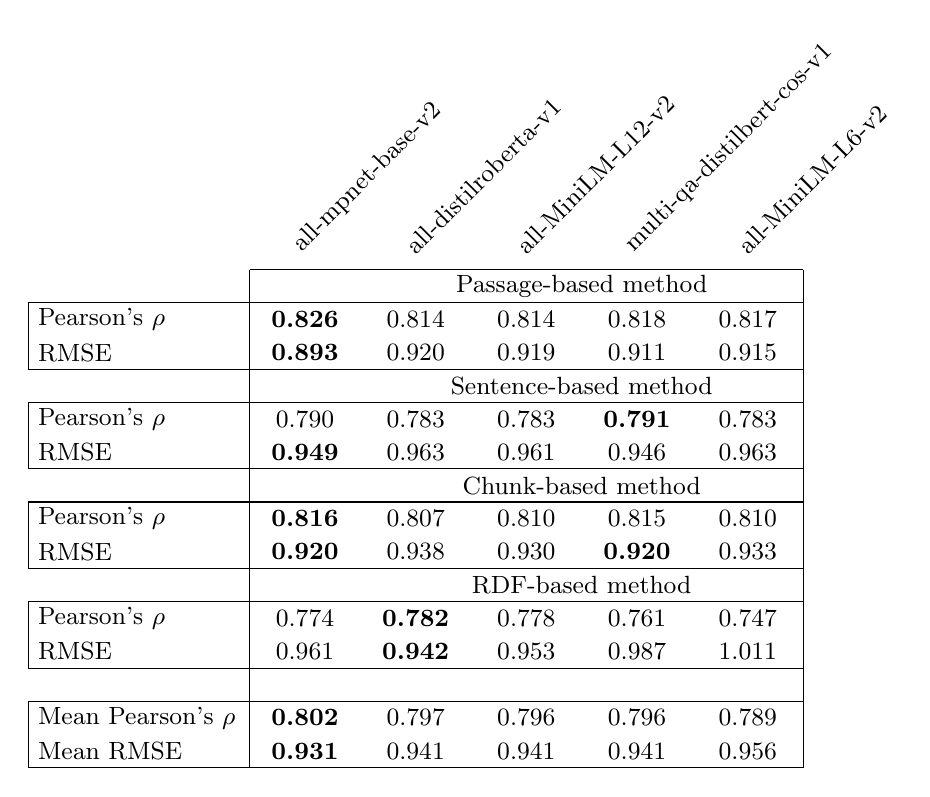
\begin{tikzpicture}
		\def\mycollabels{all-mpnet-base-v2, all-distilroberta-v1, all-MiniLM-L12-v2, multi-qa-distilbert-cos-v1,all-MiniLM-L6-v2}
		\def\myrowlabels{,Pearson's $\rho$, RMSE, ,Pearson's $\rho$, RMSE ,, Pearson's $\rho$, RMSE, ,Pearson's $\rho$, RMSE,,Mean Pearson's $\rho$,Mean RMSE}
		\def\mydata{
			{},
			{\textbf{0.826}, 0.814, 0.814, 0.818, 0.817},
			{\textbf{0.893}, 0.920, 0.919,0.911, 0.915},
			{},
			{0.790, 0.783, 0.783, \textbf{0.791}, 0.783},
			{\textbf{0.949}, 0.963, 0.961, 0.946, 0.963},
			{},
			{\textbf{0.816}, 0.807, 0.810, 0.815, 0.810},
			{\textbf{0.920}, 0.938, 0.930, \textbf{0.920}, 0.933},
			{},
			{0.774, \textbf{0.782}, 0.778, 0.761, 0.747},
			{0.961, \textbf{0.942}, 0.953, 0.987, 1.011},
			{},
			{\textbf{0.802},	0.797,	0.796,	0.796,	0.789},
			{\textbf{0.931},	0.941,	0.941,	0.941,	0.956},
		}
		\def\height{1.2em}
		\def\size{4em}
		\def\labelsize{6em}
		\def\textsize{\small}
		
		\draw (3.5*\size, -0.5*\height) node[]{\textsize Passage-based method};
		\draw (3.5*\size, -3.5*\height) node[]{\textsize Sentence-based method};
		\draw (3.5*\size, -6.5*\height) node[]{\textsize Chunk-based method};
		\draw (3.5*\size, -9.5*\height) node[]{\textsize RDF-based method};
		\draw% horizontal lines
		(0.5*\size,0) -- (5.5*\size,0)
		(-\labelsize,-1*\height) -- (5.5*\size,-1*\height)
		(-\labelsize,-3*\height) -- (5.5*\size,-3*\height)
		(-\labelsize,-4*\height) -- (5.5*\size,-4*\height)
		(-\labelsize,-6*\height) -- (5.5*\size,-6*\height)
		(-\labelsize,-7*\height) -- (5.5*\size,-7*\height)
		(-\labelsize,-9*\height) -- (5.5*\size,-9*\height)
		(-\labelsize,-10*\height) -- (5.5*\size,-10*\height)
		(-\labelsize,-12*\height) -- (5.5*\size,-12*\height)
		(-\labelsize,-13*\height) -- (5.5*\size,-13*\height)
		(-\labelsize,-15*\height) -- (5.5*\size,-15*\height);
		
		\draw% vertical lines
		(0.5*\size,0) -- (0.5*\size,-15*\height)
		(5.5*\size,0) -- (5.5*\size,-15*\height)
		(-\labelsize,-1*\height) -- (-\labelsize,-3*\height)
		% (4.5*\size,-1*\height) -- (4.5*\size,-4*\height)
		(-\labelsize,-4*\height) -- (-\labelsize,-6*\height)
		(-\labelsize,-7*\height) -- (-\labelsize,-9*\height)
		(-\labelsize,-10*\height) -- (-\labelsize,-12*\height)
		(-\labelsize,-13*\height) -- (-\labelsize,-15*\height);
		% draw row labels
		\foreach \lbl [count=\x] in \myrowlabels {
			\draw (-\labelsize, -\x*\height+0.5*\height) node[right]{\textsize \lbl};
		}
		% draw diagonal labels
		\foreach \lbl [count=\x] in \mycollabels {
			\draw (\x*\size, 0) node[above right, rotate=45]{\textsize \lbl};
		}
		
		% draw cell labels 
		\foreach \row [count=\y] in \mydata {
			\foreach \elem [count=\x] in \row {
				\draw (\x*\size, -\y*\height+0.5*\height) node[]{\textsize \elem};
			}
		}
		\end{tikzpicture}
		}
		\caption{Shows the Pearson correlation and RMSE values for the methods with each pre-trained language model when a Random Forest classifier is used on the Mohler dataset \cite{mohler-etal-2011-learning}.}
		\label{table:Score table Random forest mohler}
	\end{table}
\end{frame}
\section{Summary}
\section{Future Work}
\section{Extra Slides}
\begin{frame}{Approach}
\framesubtitle{Feature Extraction: Passage-based method}
\begin{figure}
\centering
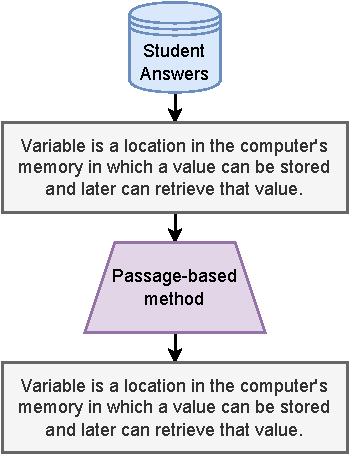
\includegraphics[scale = 0.65]{images/passage_FE.pdf}
\label{fig:passage fe}
\end{figure}
\end{frame}
\begin{frame}{Approach}
\framesubtitle{Feature Extraction: Sentence-based method}
\begin{figure}
\centering
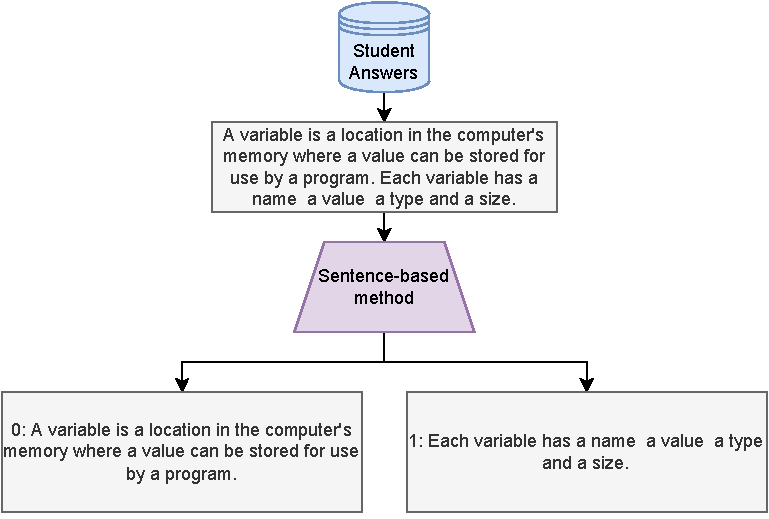
\includegraphics[scale = 0.65]{images/sentence_FE.pdf}
\label{fig:sentence fe}
\end{figure}
\end{frame}
\begin{frame}{Approach}
\framesubtitle{Feature Extraction: Chunk-based method}
\begin{figure}
\centering
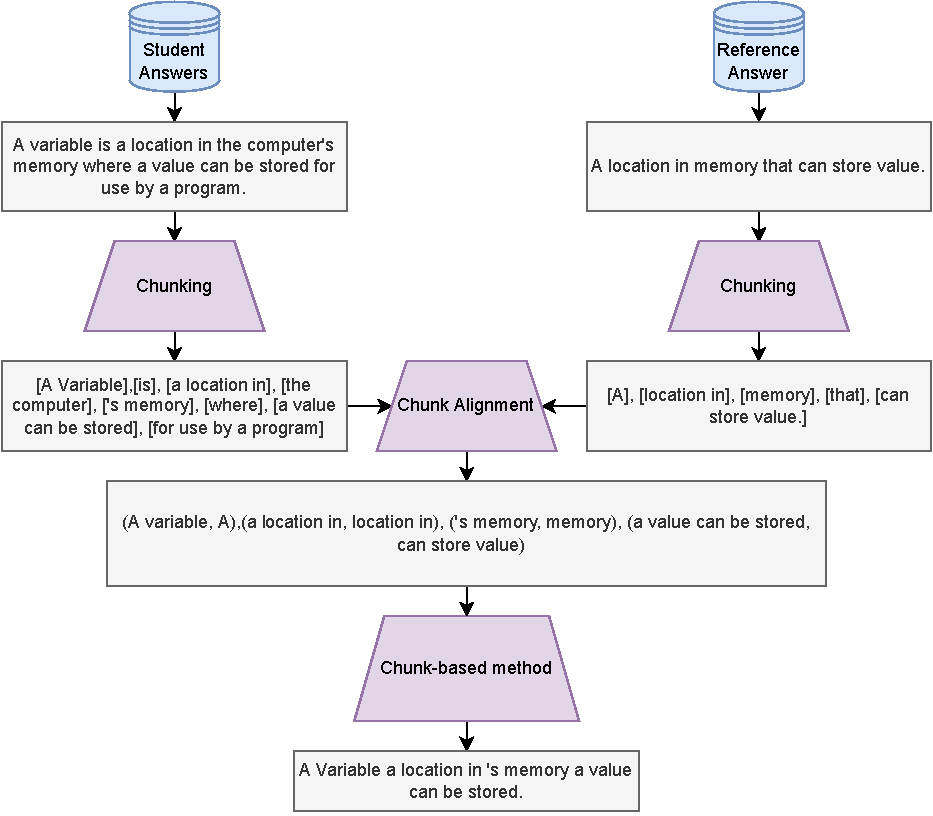
\includegraphics[scale = 0.5]{images/chunk_FE.pdf}
\label{fig:chunk fe}
\end{figure}
\end{frame}
\begin{frame}{Approach}
\framesubtitle{Feature Extraction: RDF-based method}
\begin{figure}
\centering
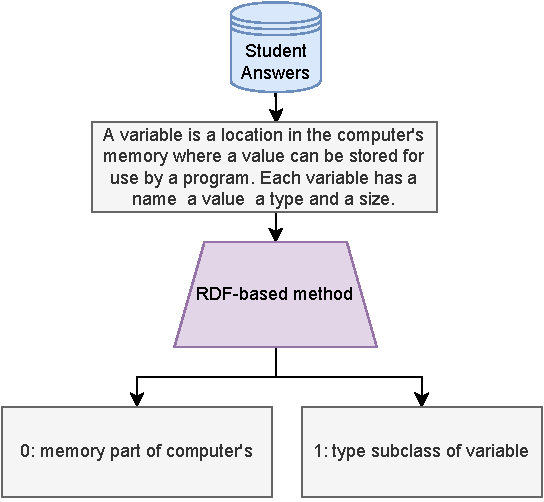
\includegraphics[scale = 0.65]{images/RDF_FE.pdf}
\label{fig:rdf fe}
\end{figure}
\end{frame}






\begin{frame}{Jabberwocky}
      \framesubtitle{Lewis Carroll}%
      \begin{tikzpicture}[overlay,remember picture]
        \node[anchor=south east,xshift=-30pt,yshift=35pt]
          at (current page.south east) {
            %\includegraphics[width=35mm]{resources/jabberwocky-light}
          };
      \end{tikzpicture}%
      'Twas brillig, and the slithy toves\\
      Did gyre and gimble in the wabe;\\
      All mimsy were the borogoves,\\
      And the mome raths outgrabe.\\\bigskip

      “Beware the Jabberwock, my son!\\
      The jaws that bite, the claws that catch!\\
      Beware the Jubjub bird, and shun\\
      The frumious Bandersnatch!”\\
\end{frame}


\begin{frame}[label=lists]{Lists and locales}
      \framesubtitle{Lorem ipsum dolor sit amet}
      \begin{columns}[onlytextwidth]
        \column{.5\textwidth}
          \begin{itemize}
            \item Nulla nec lacinia odio. Curabitur urna tellus.
            \begin{itemize}
              \item Fusce id sodales dolor. Sed id metus dui.
              \begin{itemize}
                \item Cupio virtus licet mi vel feugiat.
              \end{itemize}
            \end{itemize}
          \end{itemize}
        \column{.5\textwidth}
          \begin{enumerate}
            \item Donec porta, risus porttitor egestas scelerisque video.
            \begin{enumerate}
              \item Nunc non ante fringilla, manus potentis cario.
              \begin{enumerate}
                \item Pellentesque servus morbi tristique.
              \end{enumerate}
            \end{enumerate}
          \end{enumerate}
      \end{columns}
      \bigskip
      \justifying

      {\uselanguage{czech}Nechť již hříšné saxofony ďáblů
      rozzvučí síň úděsnými tóny waltzu, tanga a quickstepu!}
      {\uselanguage{slovak} Nezvyčajné kŕdle šťastných figliarskych
      ďatľov učia pri kótovanom ústí Váhu mĺkveho koňa Waldemara
      obžierať väč\-šie kusy exkluzívnej kôry.}
      {\uselanguage{english}The quick, brown fox jumps over a lazy
      dog. DJs flock by when MTV ax quiz prog. “Now fax quiz Jack!”}
\end{frame}

\subsection{Structuring Elements}
    \begin{frame}[label=simmonshall]{Text blocks}
      \framesubtitle{In plain, example, and \alert{alert} flavour}
      \alert{This text} is highlighted.

      \begin{block}{A plain block}
        This is a plain block containing some \alert{highlighted text}.
      \end{block}
      \begin{exampleblock}{An example block}
        This is an example block containing some \alert{highlighted text}.
      \end{exampleblock}
      \begin{alertblock}{An alert block}
        This is an alert block containing some \alert{highlighted text}.
      \end{alertblock}
    \end{frame}


\begin{frame}[label=proof]{Definitions, theorems, and proofs}
      \framesubtitle{All integers divide zero}
      \begin{definition}
        $\forall a,b\in\mathds{Z}: a\mid b\iff\exists c\in\mathds{Z}:a\cdot c=b$
      \end{definition}
      \begin{theorem}
        $\forall a\in\mathds{Z}: a\mid 0$
      \end{theorem}
      \begin{proof}[Proof\nopunct]
      	$\forall a\in \mathds{Z}:\cdot 0=0$
      \end{proof}
\end{frame}

    \subsection{Numerals and Mathematics}
    \begin{frame}[label=math]{Numerals and Mathematics}
      \framesubtitle{Formulae, equations, and expressions}
      \begin{columns}[onlytextwidth]
        \column{.20\textwidth}
          1234567890
        \column{.20\textwidth}
          \oldstylenums{1234567890}
        \column{.20\textwidth}
          $\hat{x}$, $\check{x}$, $\tilde{a}$,
         $\bar{a}$, $\dot{y}$, $\ddot{y}$
        \column{.40\textwidth}
          $\int \!\! \int f(x,y,z)\,\mathsf{d}x\mathsf{d}y\mathsf{d}z$
      \end{columns}
      \begin{columns}[onlytextwidth]
        \column{.5\textwidth}
          $$\frac{1}{\displaystyle 1+
            \frac{1}{\displaystyle 2+
            \frac{1}{\displaystyle 3+x}}} +
            \frac{1}{1+\frac{1}{2+\frac{1}{3+x}}}$$
        \column{.5\textwidth}
          $$F:\left| \begin{array}{ccc}
          F''_{xx} & F''_{xy} &  F'_x \\
          F''_{yx} & F''_{yy} &  F'_y \\
          F'_x     & F'_y     & 0
         \end{array}\right| = 0$$
      \end{columns}
      \begin{columns}[onlytextwidth]
        \column{.3\textwidth}
          $$\mathop{\int \!\!\! \int}_{\mathbf{x} \in \mathds{R}^2}
          \! \langle \mathbf{x},\mathbf{y}\rangle\,\mathsf{d}\mathbf{x}$$
        \column{.33\textwidth}
         $$\overline{\overline{a\alpha}^2+\underline{b\beta}
           +\overline{\overline{d\delta}}}$$
        \column{.37\textwidth}
          $\left] 0,1\right[ + \lceil x \rfloor - \langle x,y\rangle$
      \end{columns}
      \begin{columns}[onlytextwidth]
        \column{.4\textwidth}
          \begin{eqnarray*}
           e^x &\approx& 1+x+x^2/2! + \\
             && {}+x^3/3! + x^4/4!
          \end{eqnarray*}
        \column{.6\textwidth}
          $${n+1\choose k} = {n\choose k} + {n \choose k-1}$$
      \end{columns}
    \end{frame}

    \subsection{Figures and Code Listings}
    \begin{frame}[label=figs1]{Figures}
      \framesubtitle{Tables, graphs, and images}
      \begin{table}[!b]
%        {\carlitoTLF % Use monospaced lining figures
        \begin{tabularx}{\textwidth}{Xrrr}
          \textbf{Faculty} & \textbf{With \TeX} & \textbf{Total} &
          \textbf{\%} \\
          \toprule
          Faculty of Informatics       & 1\,716  & 2\,904  &
          59.09 \\% 1433
          Faculty of Science           & 786     & 5\,275  &
          14.90 \\% 1431
          Faculty of $\genfrac{}{}{0pt}{}{\textsf{Economics and}}{%
          \textsf{Administration}}$    & 64      & 4\,591  &
          1.39  \\% 1456
          Faculty of Arts              & 69      & 10\,000 &
          0.69  \\% 1421
          Faculty of Medicine          & 8       & 2\,014  &
          0.40  \\% 1411
          Faculty of Law               & 15      & 4\,824  &
          0.31  \\% 1422
          Faculty of Education         & 19      & 8\,219  &
          0.23  \\% 1441
          Faculty of Social Studies    & 12      & 5\,599  &
          0.21  \\% 1423
          Faculty of Sports Studies    & 3       & 2\,062  &
          0.15  \\% 1451
          \bottomrule
        \end{tabularx}%}
        \caption{The distribution of theses written using \TeX\ during 2010--15 at MU}
      \end{table}
    \end{frame}
    \begin{frame}[label=figs2]{Figures}
      \framesubtitle{Tables, graphs, and images}
      \begin{figure}[b]
        \centering
        % Flipping a coin
        % Author: cis
        \tikzset{
          head/.style = {fill = none, label = center:\textsf{H}},
          tail/.style = {fill = none, label = center:\textsf{T}}}
        \scalebox{0.65}{\begin{tikzpicture}[
            scale = 1.5, transform shape, thick,
            every node/.style = {draw, circle, minimum size = 10mm},
            grow = down,  % alignment of characters
            level 1/.style = {sibling distance=3cm},
            level 2/.style = {sibling distance=4cm},
            level 3/.style = {sibling distance=2cm},
            level distance = 1.25cm
          ]
          \node[shape = rectangle,
            minimum width = 6cm, font = \sffamily] {Coin flipping}
          child { node[shape = circle split, draw, line width = 1pt,
                  minimum size = 10mm, inner sep = 0mm, rotate = 30] (Start)
                  { \rotatebox{-30}{H} \nodepart{lower} \rotatebox{-30}{T}}
           child {   node [head] (A) {}
             child { node [head] (B) {}}
             child { node [tail] (C) {}}
           }
           child {   node [tail] (D) {}
             child { node [head] (E) {}}
             child { node [tail] (F) {}}
           }
          };

          % Filling the root (Start)
          \begin{scope}[on background layer, rotate=30]
            \fill[head] (Start.base) ([xshift = 0mm]Start.east) arc (0:180:5mm)
              -- cycle;
            \fill[tail] (Start.base) ([xshift = 0pt]Start.west) arc (180:360:5mm)
              -- cycle;
          \end{scope}

          % Labels
          \begin{scope}[nodes = {draw = none}]
            \path (Start) -- (A) node [near start, left]  {$0.5$};
            \path (A)     -- (B) node [near start, left]  {$0.5$};
            \path (A)     -- (C) node [near start, right] {$0.5$};
            \path (Start) -- (D) node [near start, right] {$0.5$};
            \path (D)     -- (E) node [near start, left]  {$0.5$};
            \path (D)     -- (F) node [near start, right] {$0.5$};
            \begin{scope}[nodes = {below = 11pt}]
              \node [name = X] at (B) {$0.25$};
              \node            at (C) {$0.25$};
              \node [name = Y] at (E) {$0.25$};
              \node            at (F) {$0.25$};
            \end{scope}
          \end{scope}
        \end{tikzpicture}}
        \caption{Tree of probabilities -- Flipping a coin\footnote[frame]{%
          A derivative of a diagram from \url{texample.net} by cis, CC BY 2.5 licensed}}
      \end{figure}
    \end{frame}

    \defverbatim[colored]\sleepSort{
      \begin{lstlisting}[language=C,tabsize=2]
  #include <stdio.h>
  #include <unistd.h>
  #include <sys/types.h>
  #include <sys/wait.h>

  // This is a comment
  int main(int argc, char **argv)
  {
          while (--c > 1 && !fork());
          sleep(c = atoi(v[c]));
          printf("%d\n", c);
          wait(0);
          return 0;
  }
    \end{lstlisting}}
    \begin{frame}{Code listings}{An example source code in C}
      \sleepSort
    \end{frame}

    \subsection{Citations and Bibliography}
    \begin{frame}[label=citations]{Citations}
      \framesubtitle{\TeX, \LaTeX, and Beamer}

      \justifying\TeX\ is a programming language for the typesetting
      of documents. It was created by Donald Erwin Knuth in the late
      1970s and it is documented in \emph{The \TeX
      book}~\cite{knuth84}.

      In the early 1980s, Leslie Lamport created the initial version
      of \LaTeX, a high-level language on top of \TeX, which is
      documented in \emph{\LaTeX : A Document Preparation
      System}~\cite{lamport94}. There exists a healthy ecosystem of
      packages that extend the base functionality of \LaTeX;
      \emph{The \LaTeX\ Companion}~\cite{MG94} acts as a guide
      through the ecosystem.

      In 2003, Till Tantau created the initial version of Beamer, a
      \LaTeX\ package for the creation of presentations. Beamer is
      documented in the \emph{User's Guide to the Beamer
      Class}~\cite{tantau04}.
    \end{frame}

    \begin{frame}[label=bibliography]{Bibliography}
      \framesubtitle{\TeX, \LaTeX, and Beamer}
      \begin{thebibliography}{9}
      	\bibitem{SBERT}
      		
        \bibitem{knuth84}
            Donald~E.~Knuth.
            \emph{The \TeX book}.
            Addison-Wesley, 1984.
        \bibitem{lamport94}
            Leslie~Lamport.
            \emph{\LaTeX : A Document Preparation System}.
            Addison-Wesley, 1986.
        \bibitem{MG94}
            M.~Goossens, F.~Mittelbach, and A.~Samarin.
            \emph{The \LaTeX\ Companion}.
            Addison-Wesley, 1994.
        \bibitem{tantau04}
            Till~Tantau.
            \emph{User's Guide to the Beamer Class Version 3.01}.
            Available at \url{http://latex-beamer.sourceforge.net}.
        \bibitem{MS05}
            A.~Mertz and W.~Slough.
            Edited by B.~Beeton and K.~Berry.
            \emph{Beamer by example} In TUGboat,
              Vol. 26, No. 1., pp. 68-73.
      \end{thebibliography}
    \end{frame}


\section{Something else}

\begin{frame}
\frametitle{There Is No Largest Prime Number}
\framesubtitle{The proof uses \textit{reductio ad absurdum}.}
\begin{theorem}
There is no largest prime number. \end{theorem}
\begin{enumerate}
\item<1-| alert@1> Suppose $p$ were the largest prime number.
\item<2-> Let $q$ be the product of the first $p$ numbers.
\item<3-> Then $q+1$ is not divisible by any of them.
\item<1-> But $q + 1$ is greater than $1$, thus divisible by some prime
number not in the first $p$ numbers.
\end{enumerate}
\end{frame}

\begin{frame}{A longer title}
\begin{itemize}
\item one
\item two

\textbf{This is a test of bold text}

\end{itemize}
\end{frame}

\begin{frame}[allowframebreaks]{Test}
  First slide
  \begin{itemize}
    \item
    \item
    \item
    \item
    \item
  \end{itemize}
  \framebreak
  Second slide
  \begin{itemize}
    \item
    \item
    \item
    \item
    \item
  \end{itemize}
\end{frame}
%--- Next Frame ---%



\end{document}
